% ==============================================================================
% Chapter 2: Market Context, Business Model, Users & Stakeholders
% Indicative Space Budget: ~2.5 pages
% Status: Draft — Prepared by Research; Pending Partner Review
% ==============================================================================

\fgchapterflow{02}{Chapter 02 --- Market \& Stakeholders}{Market Context, Business Model, Users \& Stakeholders}{Verified EV adoption context, competitor audit, ecosystem roles, and stakeholder matrix}{sec:market-stakeholders}

\subsection{Dual-Energy Market Context and Data Provenance}
\label{sec:market-context}

The commercial rationale for Fuel\&Go rests on the coexistence of legacy liquid-fuel infrastructure and rapidly expanding public EV charging networks. Directly verified 2024 global measurements from the IEA \emph{Global EV Outlook 2025}~\cite{iea2025gev} demonstrate both rapid fleet electrification and regional variation in public charging density:
\begin{itemize}[leftmargin=1.4em, itemsep=2pt]
  \item \textbf{Global Sales Momentum (\texttt{[Sourced Measurement]})}: Electric car sales (BEV and PHEV) exceeded 17~million vehicles globally in 2024---an increase of more than 25\% year-over-year compared to 2023---reaching a sales share of more than 20\% of all new cars sold worldwide~\cite{iea2025gev}.
  \item \textbf{Public Charging Coverage (\texttt{[Sourced Measurement]})}: In 2024, China had \emph{more than 1~public charger for every 10~electric cars} (a reciprocal upper bound of fewer than 10~electric cars per public charger, rather than an exact measured value of~10), whereas the European Union averaged \emph{1~public charger for every 13~electric cars}~\cite{iea2025gev}. Expanding public charging access is particularly important in dense urban areas where apartment housing limits private home charging~\cite{iea2025gev}.
  \item \textbf{Israeli Market Context (\texttt{[Unverified --- Excluded from Empirical Claims]})}: The original Fuel\&Go presentation (Slides~2 and 8) positions Israel as the primary launch market due to rising EV adoption and brand-specific app fragmentation. Because official primary-source tables from the Israel Central Bureau of Statistics (CBS) have not been directly inspected, secondary press summaries of Israeli BEV market share are classified as \emph{unverified} and strictly excluded from empirical claims, calculations, and Figure~\ref{fig:market-context}.
\end{itemize}

% ------------------------------------------------------------------------------
% FIGURE 2.1 HOOK FOR DESIGN AGENT (Reproducible Python Plot #1)
% Source CSV: data/ev_market_summary_verified.csv (iea2025gev rows ONLY;
%             strictly exclude UNVERIFIED_EXCLUDED Israel rows).
% Design Spec (Finding 1):
%   - Do NOT plot vehicle sales (millions) and percentages on a shared numerical axis.
%   - Use separate clearly labeled panels or designed KPI cards.
%   - Preserve "more than" (>) and "on average" (~) qualifiers.
%   - Do NOT plot China's ">1.0 public chargers per 10 electric cars" (<10 EVs/charger)
%     as an exact measured bar of 10.
% Required Provenance Tag in Chart & Caption: [Sourced Measurement] (+ [Calculation] if reciprocal shown)
% ------------------------------------------------------------------------------
\begin{figure}[htbp]
  \centering
  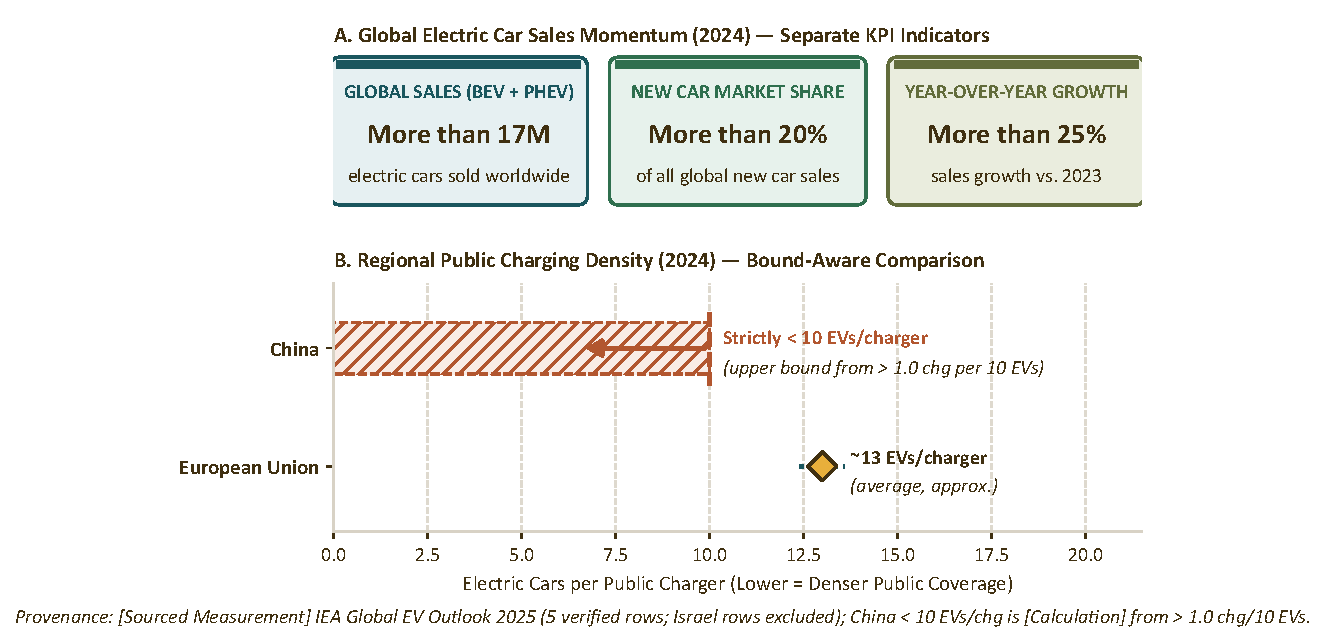
\includegraphics[width=\linewidth]{figures/fig2_1_market_context.pdf}
  \caption{Global EV Adoption and Regional Public Charging Coverage (2024). Separate panels/KPI cards avoid mixing incompatible units and preserve IEA uncertainty qualifiers (``more than'' and ``on average''). \emph{Provenance}: \texttt{[Sourced Measurement]} from IEA \emph{Global EV Outlook 2025}~\cite{iea2025gev} (Executive Summary and Electric Vehicle Charging chapters); China's reciprocal upper bound ($<10$~electric cars per public charger) is a deterministic \texttt{[Calculation]} from IEA's ``more than 1~public charger per 10~electric cars.''}
  \label{fig:market-context}
\end{figure}

\subsection{Competitive Landscape Verification}
\label{sec:competitors}

The original Fuel\&Go presentation (Slides~13, 74, and 75) defines qualitative market tiers (TAM: regular fueling/charging drivers; SAM: drivers at digitally enabled stations; SOM: EV owners and tech-savvy drivers seeking a unified app; Slide~12) and positions Fuel\&Go against navigation apps, fuel-chain apps, and EV-only network apps. Each referenced competitor was verified against official product or help documentation inspected on 2026-11-27:

\begin{itemize}[leftmargin=1.4em, itemsep=2pt]
  \item \textbf{Waze (Navigation-First Indirect Competitor)}~\cite{waze2025help,waze2025gas}: Inspected official Waze Help articles document route-based EV charging station discovery (filtered by plug type and preferred network)~\cite{waze2025help} and community-reported fuel types and gas prices~\cite{waze2025gas}. Within these official guides, Waze's documented scope centers on navigation, discovery, and crowd-sourced pricing rather than remote pump/charger activation, live energy telemetry, or unified payment settlement.
  \item \textbf{Paz \texttt{yellow} App (Brand-Centric Fuel \& Retail Competitor)}~\cite{paz2025yellow}: The inspected official Paz product page documents \texttt{yellow} as a digital wallet and cashback loyalty platform covering fueling at Paz stations, convenience-store purchases, \emph{Paz Charge} EV charging, and partner perks. \emph{Correction vs.\ Slide~74}: Although Slide~74 described \texttt{yellow}'s EV support as limited, current official documentation confirms Paz Charge integration inside \texttt{yellow}. However, the inspected page positions \texttt{yellow} around the Paz and \texttt{yellow} partner ecosystem rather than cross-operator roaming across competing fuel chains and third-party EV Charge Point Operators (CPOs).
  \item \textbf{EV-Edge~\cite{evedge2025app} and Afcon EV \texttt{ON}~\cite{afconev2025on} (EV-Focused Direct Competitors)}: The inspected official EV-Edge public charging network page and Afcon EV \texttt{ON} application page document dedicated Israeli EV charging apps offering station discovery, charger speed/connector filtering, live availability, and mobile payment. Liquid-fuel forecourt dispensing is not part of the documented offering on either inspected page.
\end{itemize}

Fuel\&Go's proposed differentiation (Slide~75) is therefore an \emph{operator-agnostic, dual-energy, end-to-end session flow} spanning discovery, remote activation, live telemetry, and settlement across both liquid-fuel forecourts and EV charging networks.

\subsection{Business Model: Established Ecosystem Roles vs.\ Proposed Mechanisms}
\label{sec:business-model}

To prevent conflating established industry standards with unvalidated commercial claims, Fuel\&Go's business model separates \emph{sourced ecosystem roles} from \emph{proposed monetization mechanisms}:

\begin{enumerate}[leftmargin=1.4em, itemsep=2pt]
  \item \textbf{Established EV Roaming Roles (\texttt{[Sourced Fact]})}: Under the Open Charge Point Interface (OCPI) specification~\cite{evroaming2025ocpi}, the EV charging value chain separates the \textbf{Charge Point Operator (CPO)}---which owns and operates physical chargers and publishes Locations, Tariffs, Sessions, and Charge Detail Records (CDRs)---from the \textbf{e-Mobility Service Provider (eMSP)}---which owns the driver-facing mobile application, authentication Tokens, and driver billing. Standardized CDRs serve as the settlement record between CPO and eMSP~\cite{evroaming2025ocpi}. In this taxonomy, Fuel\&Go operates conceptually as a multi-network eMSP extended with an analogous forecourt integration layer for liquid-fuel operators.
  \item \textbf{Proposed Revenue Mechanisms (\texttt{[Proposed Choice]})}: Building on Presentation Slides~27, 40, and 75, Fuel\&Go's candidate revenue streams are: (a)~per-transaction partner commissions or wholesale-to-retail tariff spreads settled against operator CDRs/forecourt receipts; (b)~B2B API onboarding or integration fees for multi-sided ecosystem partners; and (c)~future subscription tiers for frequent drivers or fleet accounts (\texttt{EXT-03}, roadmap only). No fee percentages, unit margins, partner agreements, or profitability projections are assumed or claimed.
  \item \textbf{Major Cost Drivers \& Feasibility Constraints (\texttt{[Assumption]})}: Operating an aggregator platform entails Payment Service Provider (PSP) processing fees, cloud and real-time telemetry infrastructure, per-operator adapter onboarding and maintenance, security/PCI compliance overhead, customer acquisition cost (CAC), and driver support. Primary commercial feasibility risks include multi-operator onboarding friction and thin retail fuel margins.
\end{enumerate}

\subsection{Report Audience vs.\ System Users and Stakeholders}
\label{sec:users-stakeholders}

Following \texttt{PRD.md} (Sec.~1.3), this report separates \emph{report readers} (academic evaluators and, provisionally, executive and product/engineering decision-makers) from \emph{Fuel\&Go application users}. Within the Fuel\&Go system itself, core end users are \textbf{ICE/Hybrid Vehicle Drivers} and \textbf{EV Drivers} (including accessibility-challenged drivers highlighted on Presentation Slide~4), while external operational stakeholders comprise Fuel Station Operators, EV CPOs, and Payment Service Providers. Fleet managers (\texttt{EXT-03}) and standalone station-operator dashboards (\texttt{EXT-05}) remain outside core scope pending formal scope sign-off. Table~\ref{tab:commercial-stakeholders} consolidates the commercial overview and stakeholder roles.

\begin{table}[htbp]
  \centering
  \caption{Fuel\&Go Commercial Overview, Feasibility Constraints, and Stakeholder Matrix.}
  \label{tab:commercial-stakeholders}
  \small
  \begin{tabularx}{\linewidth}{@{}P{30mm} L P{34mm} P{26mm}@{}}
    \toprule
    \rowcolor{fgOlive}
    \fgtableheader{Dimension / Actor} & \fgtableheader{Role, Mechanism, or Core Concern} & \fgtableheader{Provenance / Basis} & \fgtableheader{Scope / Status} \\
    \midrule
    \textbf{ICE / Hybrid Driver} & Discovers stations with live prices, selects compatible fuel grade, authorizes pump, pays contactlessly, receives digital receipt. & \texttt{PRD.md} Sec.~1.3; Slides~2, 4, 50. & Core End User \\
    \textbf{EV Driver} & Filters compatible connectors/kW ratings, checks live charger status, initiates/stops charging, monitors kWh/SoC, pays contactlessly. & \texttt{PRD.md} Sec.~1.3; Slides~2, 4, 40. & Core End User \\
    \textbf{EV CPO / Roaming Partner} & Operates chargers/CSMS; publishes Locations, Tariffs, Sessions, and CDRs over OCPI~\cite{evroaming2025ocpi} to Fuel\&Go (eMSP role). & \texttt{[Sourced Fact]} OCPI~\cite{evroaming2025ocpi}; Slide~27. & External System Stakeholder \\
    \textbf{Fuel Forecourt Operator} & Operates physical dispensers and forecourt controller/POS gateway; enforces local hardware safety interlocks. & \texttt{PRD.md} Sec.~2.1; IFSF~\cite{ifsf_specs}; Slide~8. & External System Stakeholder \\
    \textbf{Payment Service Provider (PSP)} & Vaults payment credentials, issues surrogate tokens, executes pre-authorization holds, final capture, and hold release. & \texttt{[Sourced Fact]} PCI DSS~\cite{pcissc2024pcidss401}. & External System Stakeholder \\
    \midrule
    \textbf{Revenue Mechanisms} & Candidate per-transaction partner commission, B2B API integration fees, and post-MVP fleet/driver subscriptions. & \texttt{[Proposed Choice]} Slides~27, 40, 75. & Conceptual (No invented financials) \\
    \textbf{Cost Drivers \& Constraints} & PSP fees, cloud/telemetry hosting, operator onboarding/maintenance, security/compliance audits, CAC; margin sensitivity. & \texttt{[Assumption]} Industry context. & Feasibility Constraint \\
    \textbf{Product Success KPIs} & Monthly Active Users (MAU), end-to-end flow completion rate, repeat usage, active ecosystem partners, payment volume. & Presentation Slides~27, 78. & Numeric targets provisional \\
    \bottomrule
  \end{tabularx}
\end{table}
